\chapter{Tutorial Membuat Aplikasi Bisnis Model Kanvas dengan APEX}
Bagaimanasih Cara membuat Aplikasi Bisnis Model Kanvas menggunakan Apex

\section{Tutorial APEX}

\begin{enumerate}
\item Pertama, kita buat dahulu \textit{workspace} di website \url{https://apex.oracle.com/en/} 

\item Lalu, isi semua data dengan benar,kemudian login ke dalam workspace 
\begin{figure}[H]
\centering
\caption{Halaman Utama Workspace}
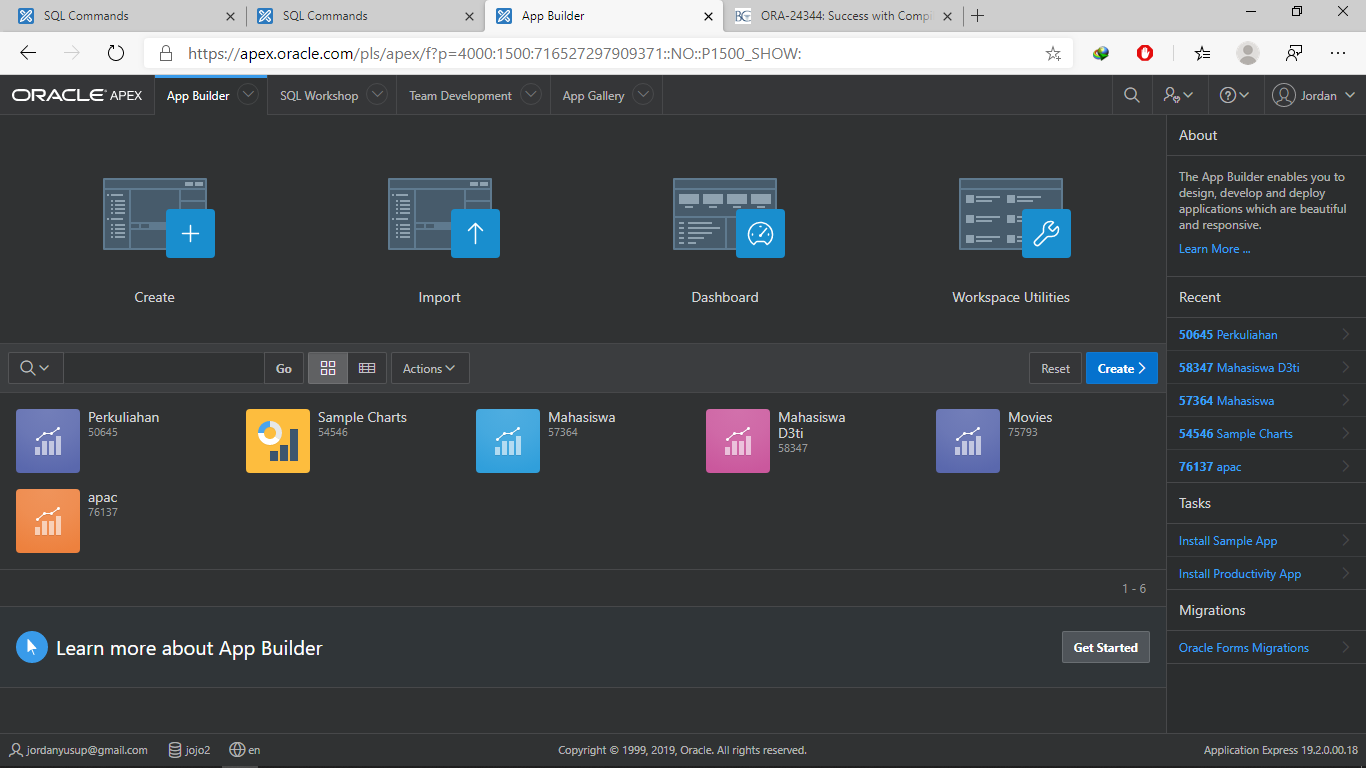
\includegraphics[width=1\textwidth]{figures/1.png}
\end{figure}

\item Sebelum membuat aplikasi kita harus mempersiapkan database yang dibutuhkan. Kita klik menu bar sql workshop lalu pilih sql commands 
\begin{figure}[H]
\centering
\caption{SQL Commands}
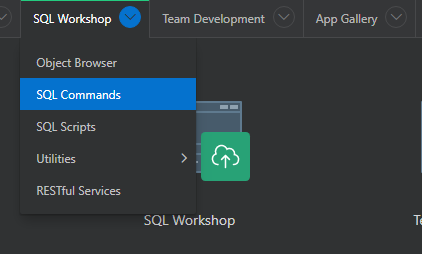
\includegraphics[witdh=1\textwidth]{figures/13.png}
\end{figure}

\item Selanjutnya, Kita membuat sebuah 5 dengan beberapa atribut 
\item Yang pertama kita membuat tabel users beserta atributnya dan id user sebagai primary key
\begin{figure}[H]
\centering
\caption{Tabel User}
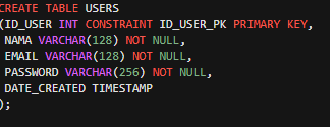
\includegraphics[witdh=1\textwidth]{figures/25.png}
\end{figure}

\item Kemudian Kita membuat tabel deskripsi bisnis. dimana di tabel ini kita memiliki 2 key yaitu id bisnis sebagai primary key dan id user sebagai foreign key. sehingga kita mengetahui data ini milik user yang mana
\begin{figure}[H]
\centering
\caption{Tabel Bisnis}
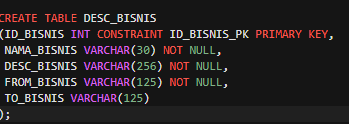
\includegraphics[witdh=1\textwidth]{figures/26.png}
\end{figure}

\item Antara Tabel BMC dan tabel binis ini saling memiliki ketergantungan. Karena tanpa bisnis yang jelas kita tidak bisa membuat atau mengisi bmc. dan jika tertuksr atau tidak sesuai maka data akan rusak.
\begin{figure}[H]
\centering
\caption{Tabel BMC}
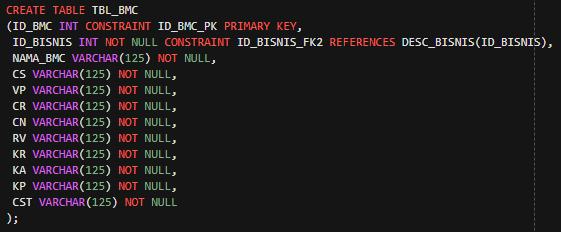
\includegraphics[witdh=1\textwidth]{figures/27.png}
\end{figure}

\item Setelah membuat tabel bmc kita harus menuntaskan dengan menghubungkan datanya ke tabel swot. dimana tabel bmc tidak akan sempurna jika tidak berpasangan dengan tabel swot
\begin{figure}[H]
\centering
\caption{Tabel SWOT}
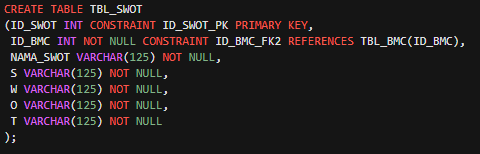
\includegraphics[witdh=1\textwidth]{figures/28.png}
\end{figure}

\item Selanjutnya kita membuat tabel analisis yang berisi tentang rangkuman dari tabel bisnis sampai tabel swot. disini kita tidak memasukan tabel user karena tabel user itu tidak boleh diketahui oleh siapapun kecuali user tersebut. 
\begin{figure}[H]
\centering
\caption{Tabel Analisis}
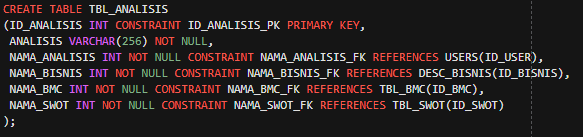
\includegraphics[witdh=1\textwidth]{figures/29.png}
\end{figure}

\item Terakhir kita membuat sebuah trigger yang di gunakan untuk menyimpan perubahan yang dilakukan oleh user secara otomatis sehingga ketika user membutuhkan data yang diubah atau dihapus kita masih menyimpan data tersebut. 
\begin{figure}[H]
\centering
\caption{SQL Commands}
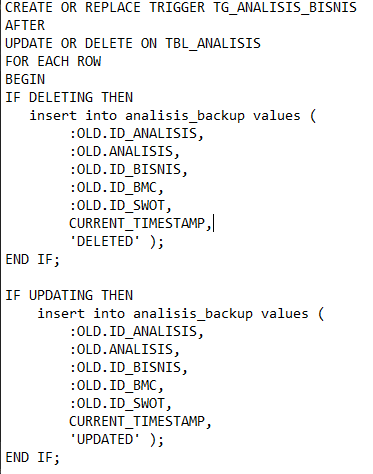
\includegraphics[witdh=1\textwidth]{figures/30.png}
\end{figure}


\item Setelah tabel yang dibutuhkan selesai kita kembali ke main menu lalu pilih \textit{app builder} dan klik create  
\begin{figure}[H]
\centering
\caption{Halaman App Builder}
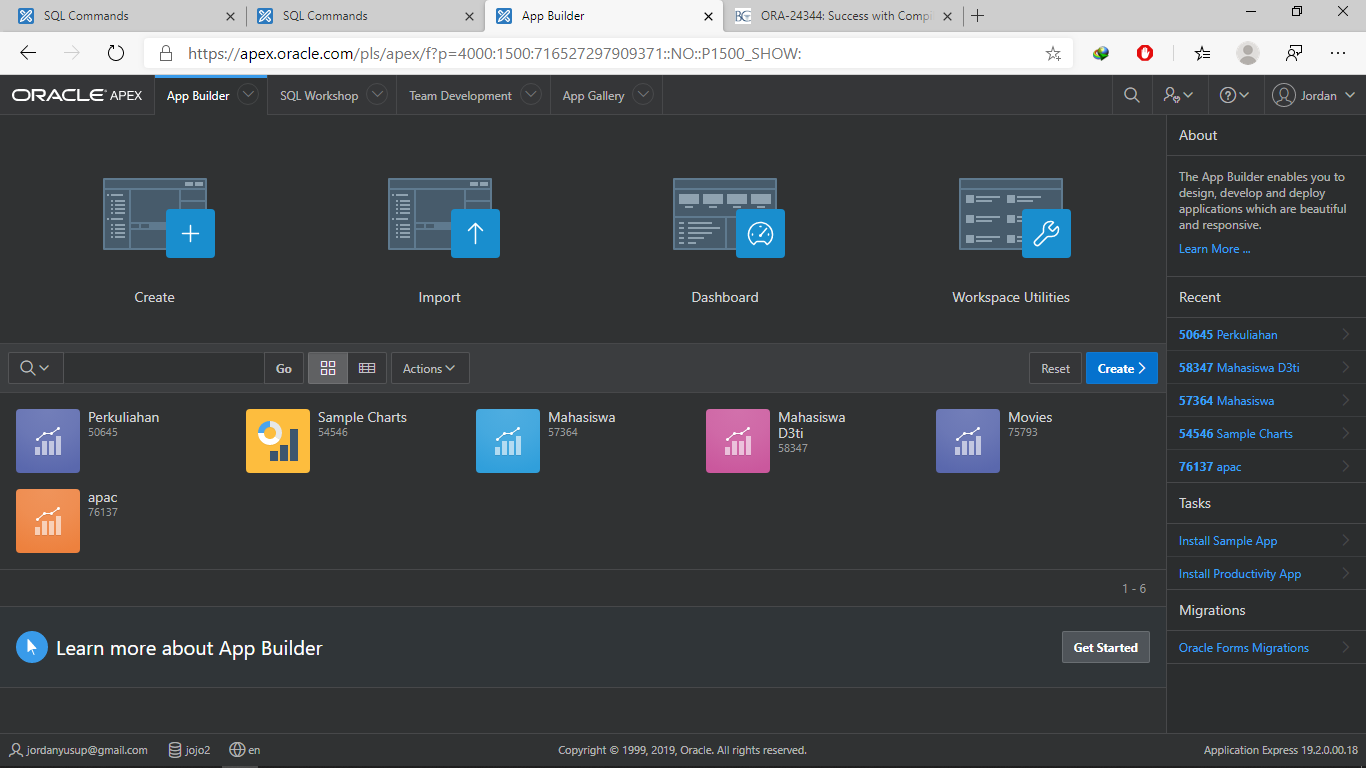
\includegraphics[width=1\textwidth]{figures/1.png}
\end{figure}

\item Selanjutnya, pilih new application
\begin{figure}[H]
\centering
\caption{Halaman Upload File}
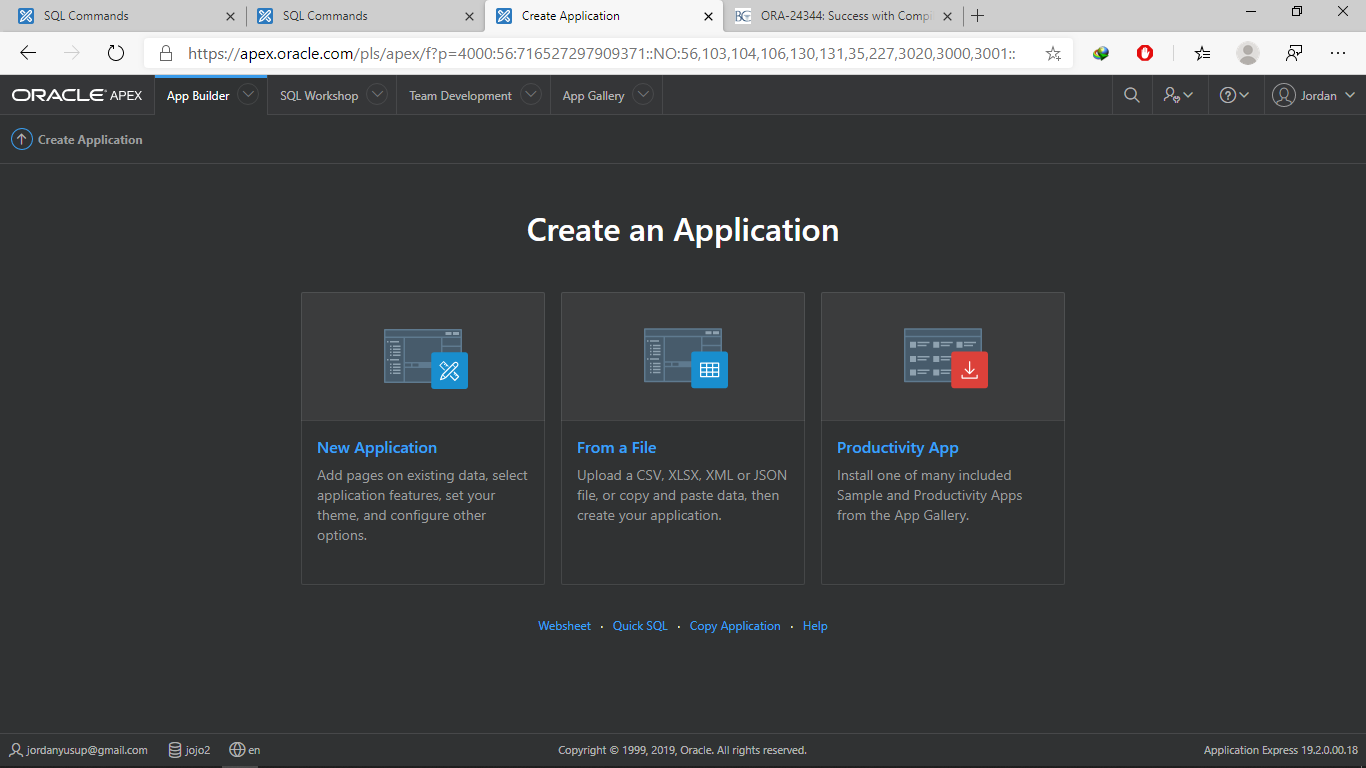
\includegraphics[width=1\textwidth]{figures/2.png}
\end{figure}


\item Kemudian pilih add page
\begin{figure}[H]
\centering
\caption{Add Page}
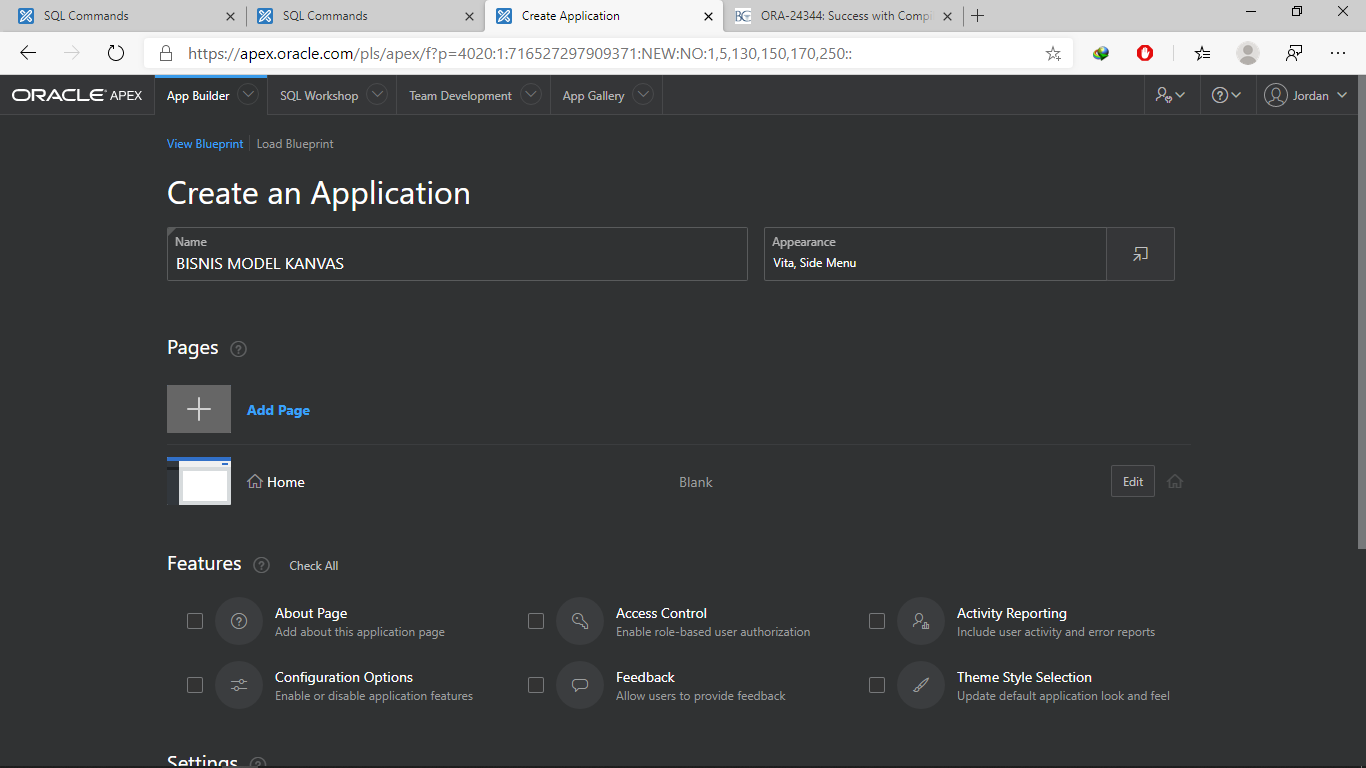
\includegraphics[width=1\textwidth]{figures/3.png}
\end{figure}

\item Pilih interactive report
\begin{figure}[H]
\centering
\caption{Interactive Report}
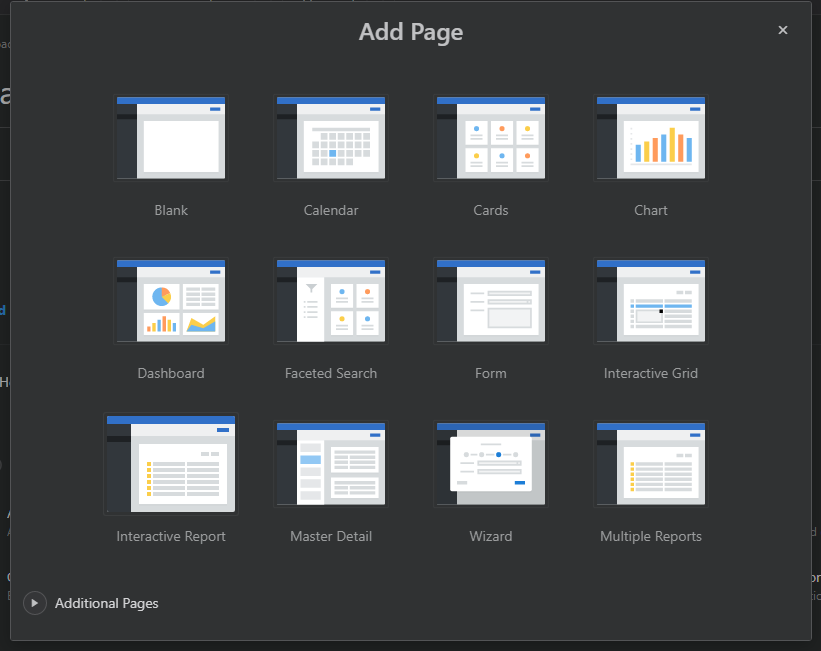
\includegraphics[width=1\textwidth]{figures/24.png}
\end{figure}

\item Klik select table, dan pilih tabelnya
\begin{figure}[H]
\centering
\caption{Pilih Tabel}
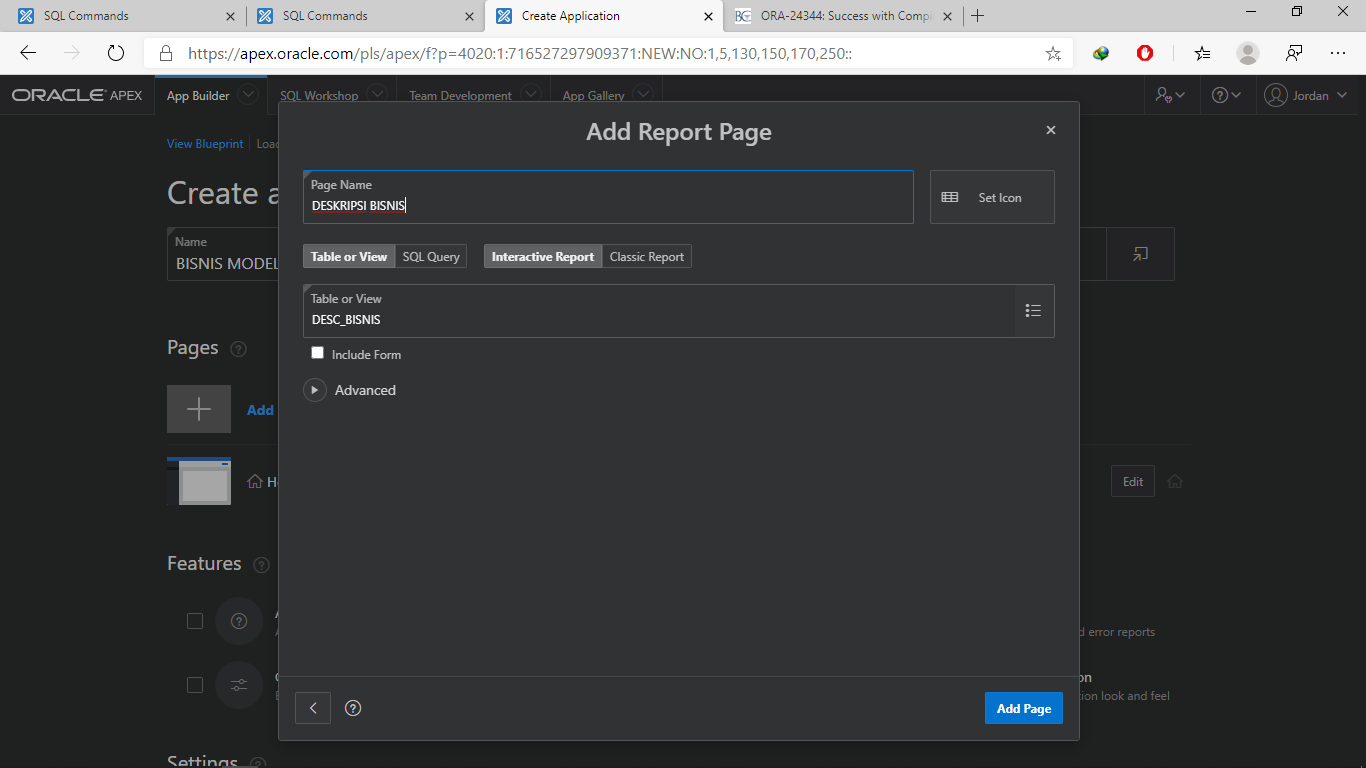
\includegraphics[width=1\textwidth]{figures/4.png}
\end{figure}

\item Kemudian isi page name lalu klik ok
\begin{figure}[H]
\centering
\caption{Isi Page Name}
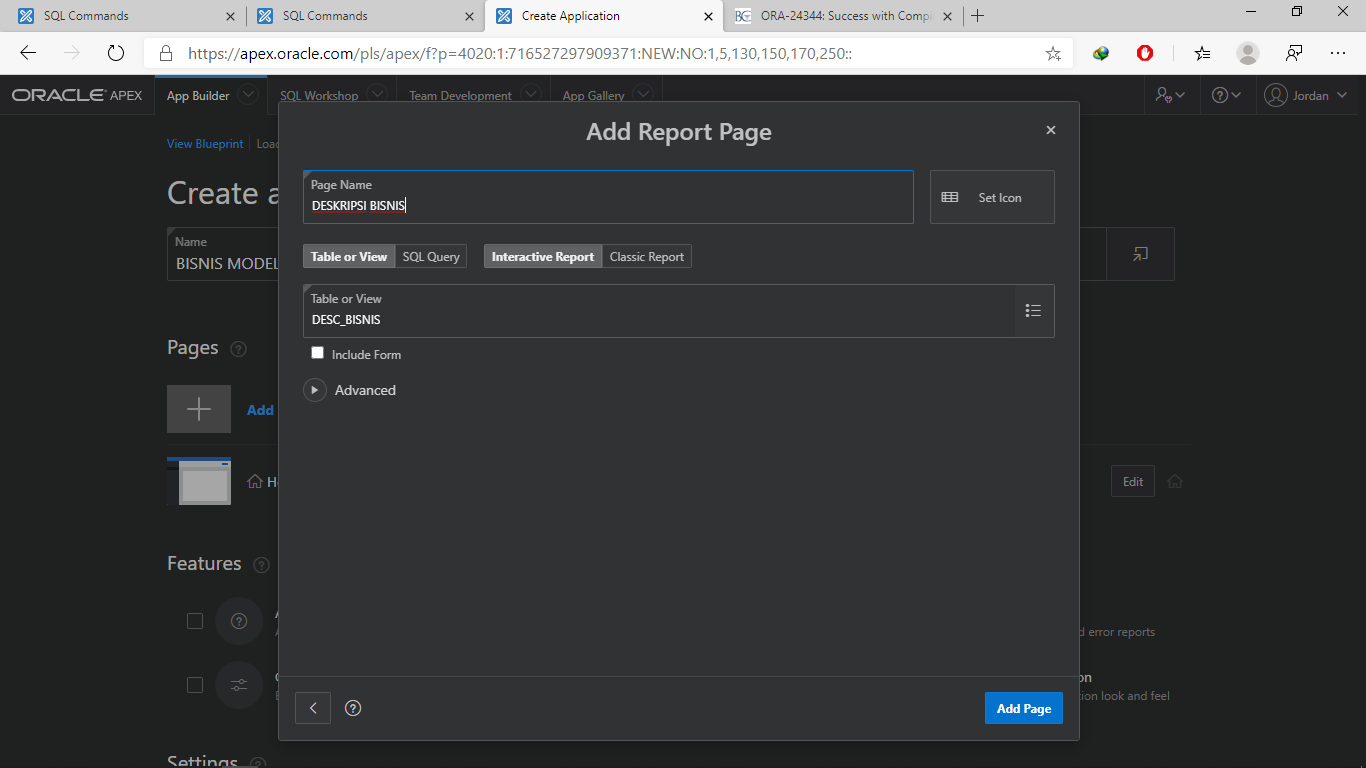
\includegraphics[width=1\textwidth]{figures/4.png}
\end{figure}

\item Ulangi langkah tersebut sesuai kebutuhan.

\item scroll kebawah lalu klik create application

\item Kemudian run application seperti gambar
\begin{figure}[H]
\centering
\caption{Run Application}
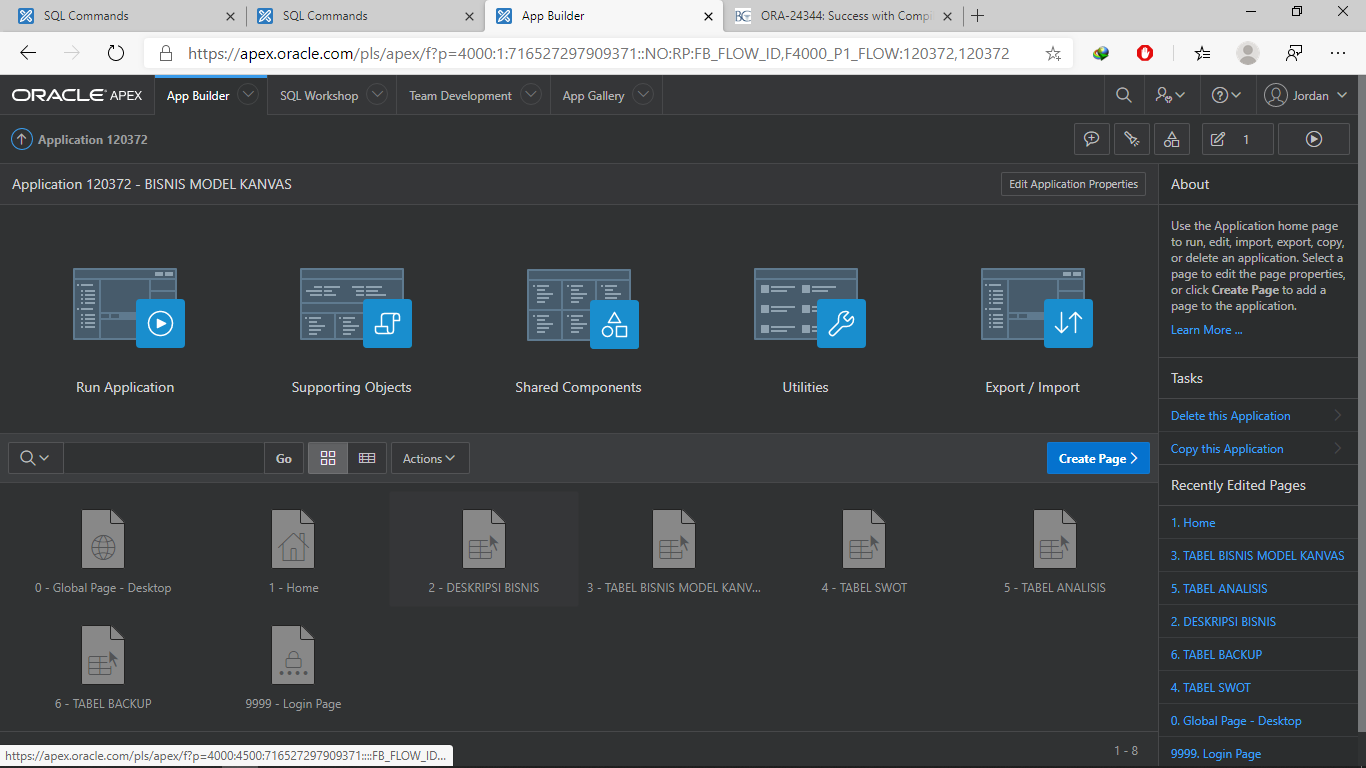
\includegraphics[width=1\textwidth]{figures/6.png}
\end{figure}

\item Hasilnya seperti ini
\begin{figure}[H]
\centering
\caption{Hasil 2}
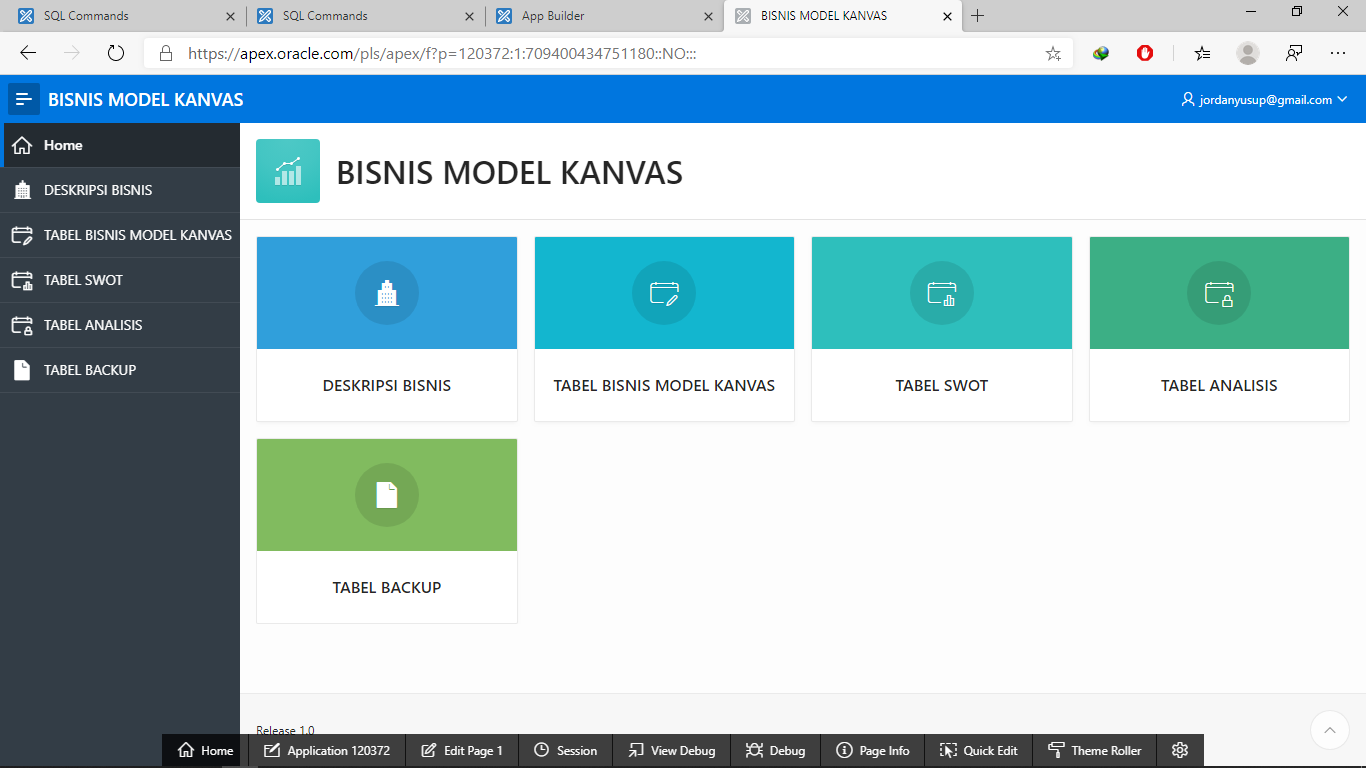
\includegraphics[width=1\textwidth]{figures/8.png}
\end{figure}
